\documentclass[
	aspectratio=169,	% Modern aspect ratio (TODO: Other ratios not yet supported)
	onlytextwidth,		% Sets totalwidth=\textwidth and therefore e.g. columns won't invade the margins
	t,					% Default vertical alignment of frames and colums at top (default is centered) % Stored in \beamer@centered (\beamer@centeredfalse, \beamer@centeredtrue)
%	handout,			% Create a basic handout of the presentation (removes overlays)
	]{beamer}


%%%%%%%%%%%%%%%%%%%%%%%%%%%%%%%%%%%%%%%%%%
% 1) Load the desired presentation theme
\usetheme[
% Individual options to customize the presentation conforming to the corporate design
hs,					% Change default faculty color set and predefined faculty values: hs or <empty> (default), inw, cb, me, sw, wi, inst (\renewcommand{\insertfacultyname}{Institutname} needed)
faculty=cb,
%	language=english,	% Change language to english (default: ngerman), other languages are possible (see babel-package) but may need further adjustments 
%	toc,				% Adds a ToC slide
%	sectionslide,		% Display separate section slides
%	subsectionslide,		% Display separate subsection slides containing section and subsection name
%	smallpagenumber,	% Reduces the size of the page number
%	nototalpages,		% Hides the total number of slide in footline
%	nofacultyicon,		% Hides the faculty icon on title page
colormath=nottext,	% Enables coloring of math text: off or <empty>, full, nottext (default)
%	printhandout,		% Places two slides on a single a4 paper for printing the presentation (beamer class option 'handout' needed)
%	noframesubtitle,	% Disables frame subtitles alltogether and slightly increases frame height
% Additional style options not completely conforming to the corporate design
%	titlepagedate,		% Shows the date on the titelpage
%	fancystyle,			% Enables some fancy styles, that are not part of the corporate design specifications (default: off)
%	progressbar,		% Shows the progressbar in footline (run twice to update progressbar)
]{hsmw} 

%%%%%%%%%%%%%%%%%%%%%%%%%%%%%%%%%%%%%%%%%%
% 2) Specify default fields for presentation and pdf document properties
% Set the title: \title{Long title everywhere} or \title[Short title for footline]{Long title for titlepage}
\title{Evaluierung von KI-basierten Modellen zur automatisierten Schwachstellenanalyse im Rahmen von Penetrationstests}
% Authors (separate multiple author names e.g. with \and for additional space): \author{author for everywhere} or \author[author for footline]{author for titlepage and thankyouslide}
\author[xxx]{xxx}
% Institute (will be prefilled automatically, depending on chosen faculty theme option): \institute{institute for everywhere} or \institute[institute for footline and thankyouslide]{institute for titlepage}
%\institute[institute for footline and thankyouslide]{institute for titlepage}
% Date of presentation (\today or a fixed value): \date{date for everywhere} or \date[date for footline]{date for titlepage}
%\date{\today} % 22. März 2022
% Impressum for thankyou slide (leave one empty if not wanted or needed):
%\email{schildba@hs-mittweida.de} % \email{E-Mail}
%\phone{+49 3727 58-1598} % \phone[Mobile Number]{Telephone Number}
%\office{Haus 8 | Richard Stücklen-Bau | Raum 8-207\newline Am Schwanenteich 6b | 09648 Mittweida} % \office{Office}
%\courseofstudies{Informatik (IF10w1-M)} % \courseofstudies{Course of Studies (Group Number)}
%\additional[Sidebar Text]{Main Text} % Additional information you may want to give (Department, Module, etc.) \additional[Sidebar Text]{Main Text}

%%%%%%%%%%%%%%%%%%%%%%%%%%%%%%%%%%%%%%%%%%
% 3) Use features
% Titlegraphic changes the title page to "wide" (default) if left empty or inserts given image (by file path) and scales to 6.2cm height otherwise:
\titlegraphic{} %\titlegraphic{figures/thankyou.jpg}

%%%%%%%%%%%%%%%%%%%%%%%%%%%%%%%%%%%%%%%%%%
% 4) Add bibliography
% Load the package and options you like, e.g. for recommended ieee style in combination of biblatex and biber:
%\usepackage[backend=biber, bibstyle=ieee, citestyle=numeric-comp, sorting=none, natbib=true, hyperref=true, dashed=false]{biblatex}
% Add your bibliography file(s)
%\addbibresource{literature.bib} 
% Dont forget to use \makebibliography where you want to put it, e.g. at the end of your presentation, after the "normal" slides:
% \appendix
% \makebibliography
% Compile with following command sequence to fully include bibliography: pdflatex, biber, pdflatex, pdflatex

%%%%%%%%%%%%%%%%%%%%%%%%%%%%%%%%%%%%%%%%%%
% 5) Existing macro usage examples

% \appendix is used as end marker for slides (slide numbers and progressbar)
% \makethankyou creates a thank you slide and is used as end marker for slides (progressbar)
% \makebibliography creates one or multiple bibliography slides

% For multiple speakers you can use \setcurrentspeaker{speaker name} or \setcurrentspeaker*{speaker name} prior to the frame
% To reset to the default author, use \resetcurrentspeaker{} or \resetcurrentspeaker*{}
% Starred versions of these macros prepend the word "speaker"

%%%%%%%%%%%%%%%%%%%%%%%%%%%%%%%%%%%%%%%%%%
% 6) Import additional packages you need, (re-)define macros and create a wonderful latex presentation

% You can remove this package - it is only needed for the dummy content
\usepackage{blindtext}
\usepackage{pifont}

%%%%%%%%%%%%%%%%%%%%%%%%%%%%%%%%%%%%%%%%%%
\begin{document}

% Folie 2 – Problemstellung & Motivation
\begin{frame}[fragile]{Problemstellung \& Motivation (1/2)}{Problemstellung}
	\begin{itemize}
		\item Pentests sind etabliert, aber teuer \& aufwendig  
		\begin{itemize}
			\item hoher Zeitaufwand
			\item Bedarf an Fachwissen
			\item kostenintensiv
		\end{itemize}
		
		\item Wachsende Angriffsflächen  
		\begin{itemize}
			\item Cloud
			\item Microservices
			\item DevOps erhöhen Komplexität und Angriffsrisiko
		\end{itemize}
		
		\item Limitierungen klassischer Methoden  
		\begin{itemize}
			\item rein manuelle Tests skalieren nicht mehr
			\item Ergebnisse abhängig von Erfahrung einzelner Tester
		\end{itemize}
	\end{itemize}
\end{frame}




% Folie 2 – Fachkräftemangel als Motivation
\begin{frame}{Fachkräftemangel als Motivation}
	\centering
	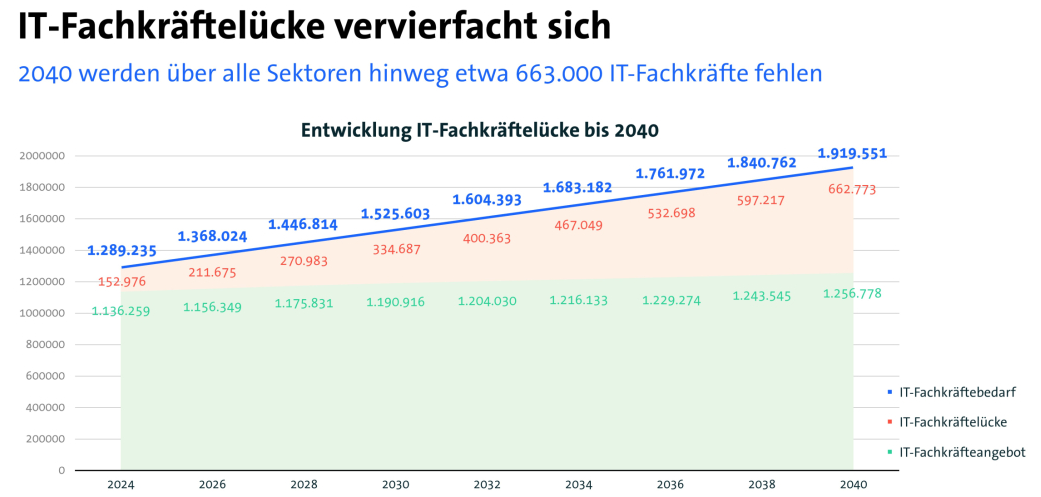
\includegraphics[width=0.65\textwidth]{figures/1.png}
	\captionof{figure}{Bitkom: IT-Fachkräftelücke bis 2040}
	\label{fig:bitkom}
\end{frame}



% Folie 3 – Ziel der Arbeit
\begin{frame}{Ziel der Arbeit}
	\textbf{Forschungsfrage:}  
	Wie können KI-Tools Sicherheitsexperten in Penetrationstests unterstützen und entlasten?	
	
	\textbf{Vorgehen:}
	\begin{itemize}
		\item Untersuchung von drei Tools:
		\begin{itemize}
			\item RamiGPT (Privilege Escalation)
			\item PentestGPT CLI (strukturierte Webtests)
			\item PentestGPT Web (dialogorientierte Tests)
		\end{itemize}
	\end{itemize}
	\textbf{Teilziele:}
	\begin{itemize}
		\item Entwicklung eines praxisnahen Bewertungsrahmens
		\item Durchführung reproduzierbarer Praxistests
		\item Vergleich: Stärken, Schwächen \& Einsatzpotenziale
	\end{itemize}
\end{frame}

% Folie – Grundlagen: Penetrationstests
\begin{frame}{Grundlagen – Penetrationstests}
	\begin{itemize}
		\item \textbf{Definition:} Gezielte Simulation von Angriffen auf IT-Systeme
		\item \textbf{Zweck:} Schwachstellen frühzeitig finden \& Sicherheitsniveau bewerten
		\item \textbf{Abgrenzung:} Unterschied zu reinen Scans $\rightarrow$ kreatives, manuelles Vorgehen
		\item \textbf{Arten:}
		\begin{itemize}
			\item Black-Box (keine Vorkenntnisse)
			\item Grey-Box (teilweise Infos)
			\item White-Box (vollständige Infos)
		\end{itemize}
	\end{itemize}
\end{frame}

% Folie – Grundlagen: Phasenmodell nach BSI
\begin{frame}{Grundlagen – Phasenmodell nach BSI}
	\begin{itemize}
		\item \textbf{Vorbereitung:} Scope, Ziele \& Rahmenbedingungen definieren
		\item \textbf{Informationsbeschaffung:} Scans, OSINT, Reconnaissance
		\item \textbf{Analyse \& Bewertung:} Identifikation \& Bewertung möglicher Schwachstellen
		\item \textbf{Exploitation:} Gezielte Ausnutzung, um Ausnutzbarkeit realistisch einzuschätzen
		\item \textbf{Abschluss \& Reporting:} Ergebnisse dokumentieren \& Empfehlungen ableiten
	\end{itemize}
\end{frame}

% Folie 4 – Penetrationstests
\begin{frame}{Grundlage (1/4)}{Penetrationstests}
	\begin{columns}
			% Linke Spalte: Text
			\begin{column}[T]{.55\textwidth}
				\begin{itemize}
					\item Ziel: Schwachstellen finden, bevor Angreifer sie ausnutzen
					\item BSI-Phasenmodell:
					\begin{enumerate}
						\item Vorbereitung
						\item Informationsbeschaffung
						\item Analyse \& Bewertung
						\item Exploitation
						\item Abschluss \& Reporting
					\end{enumerate}
				\end{itemize}
		
		\end{column}
		\begin{column}[T]{.5\textwidth}
			\centering
			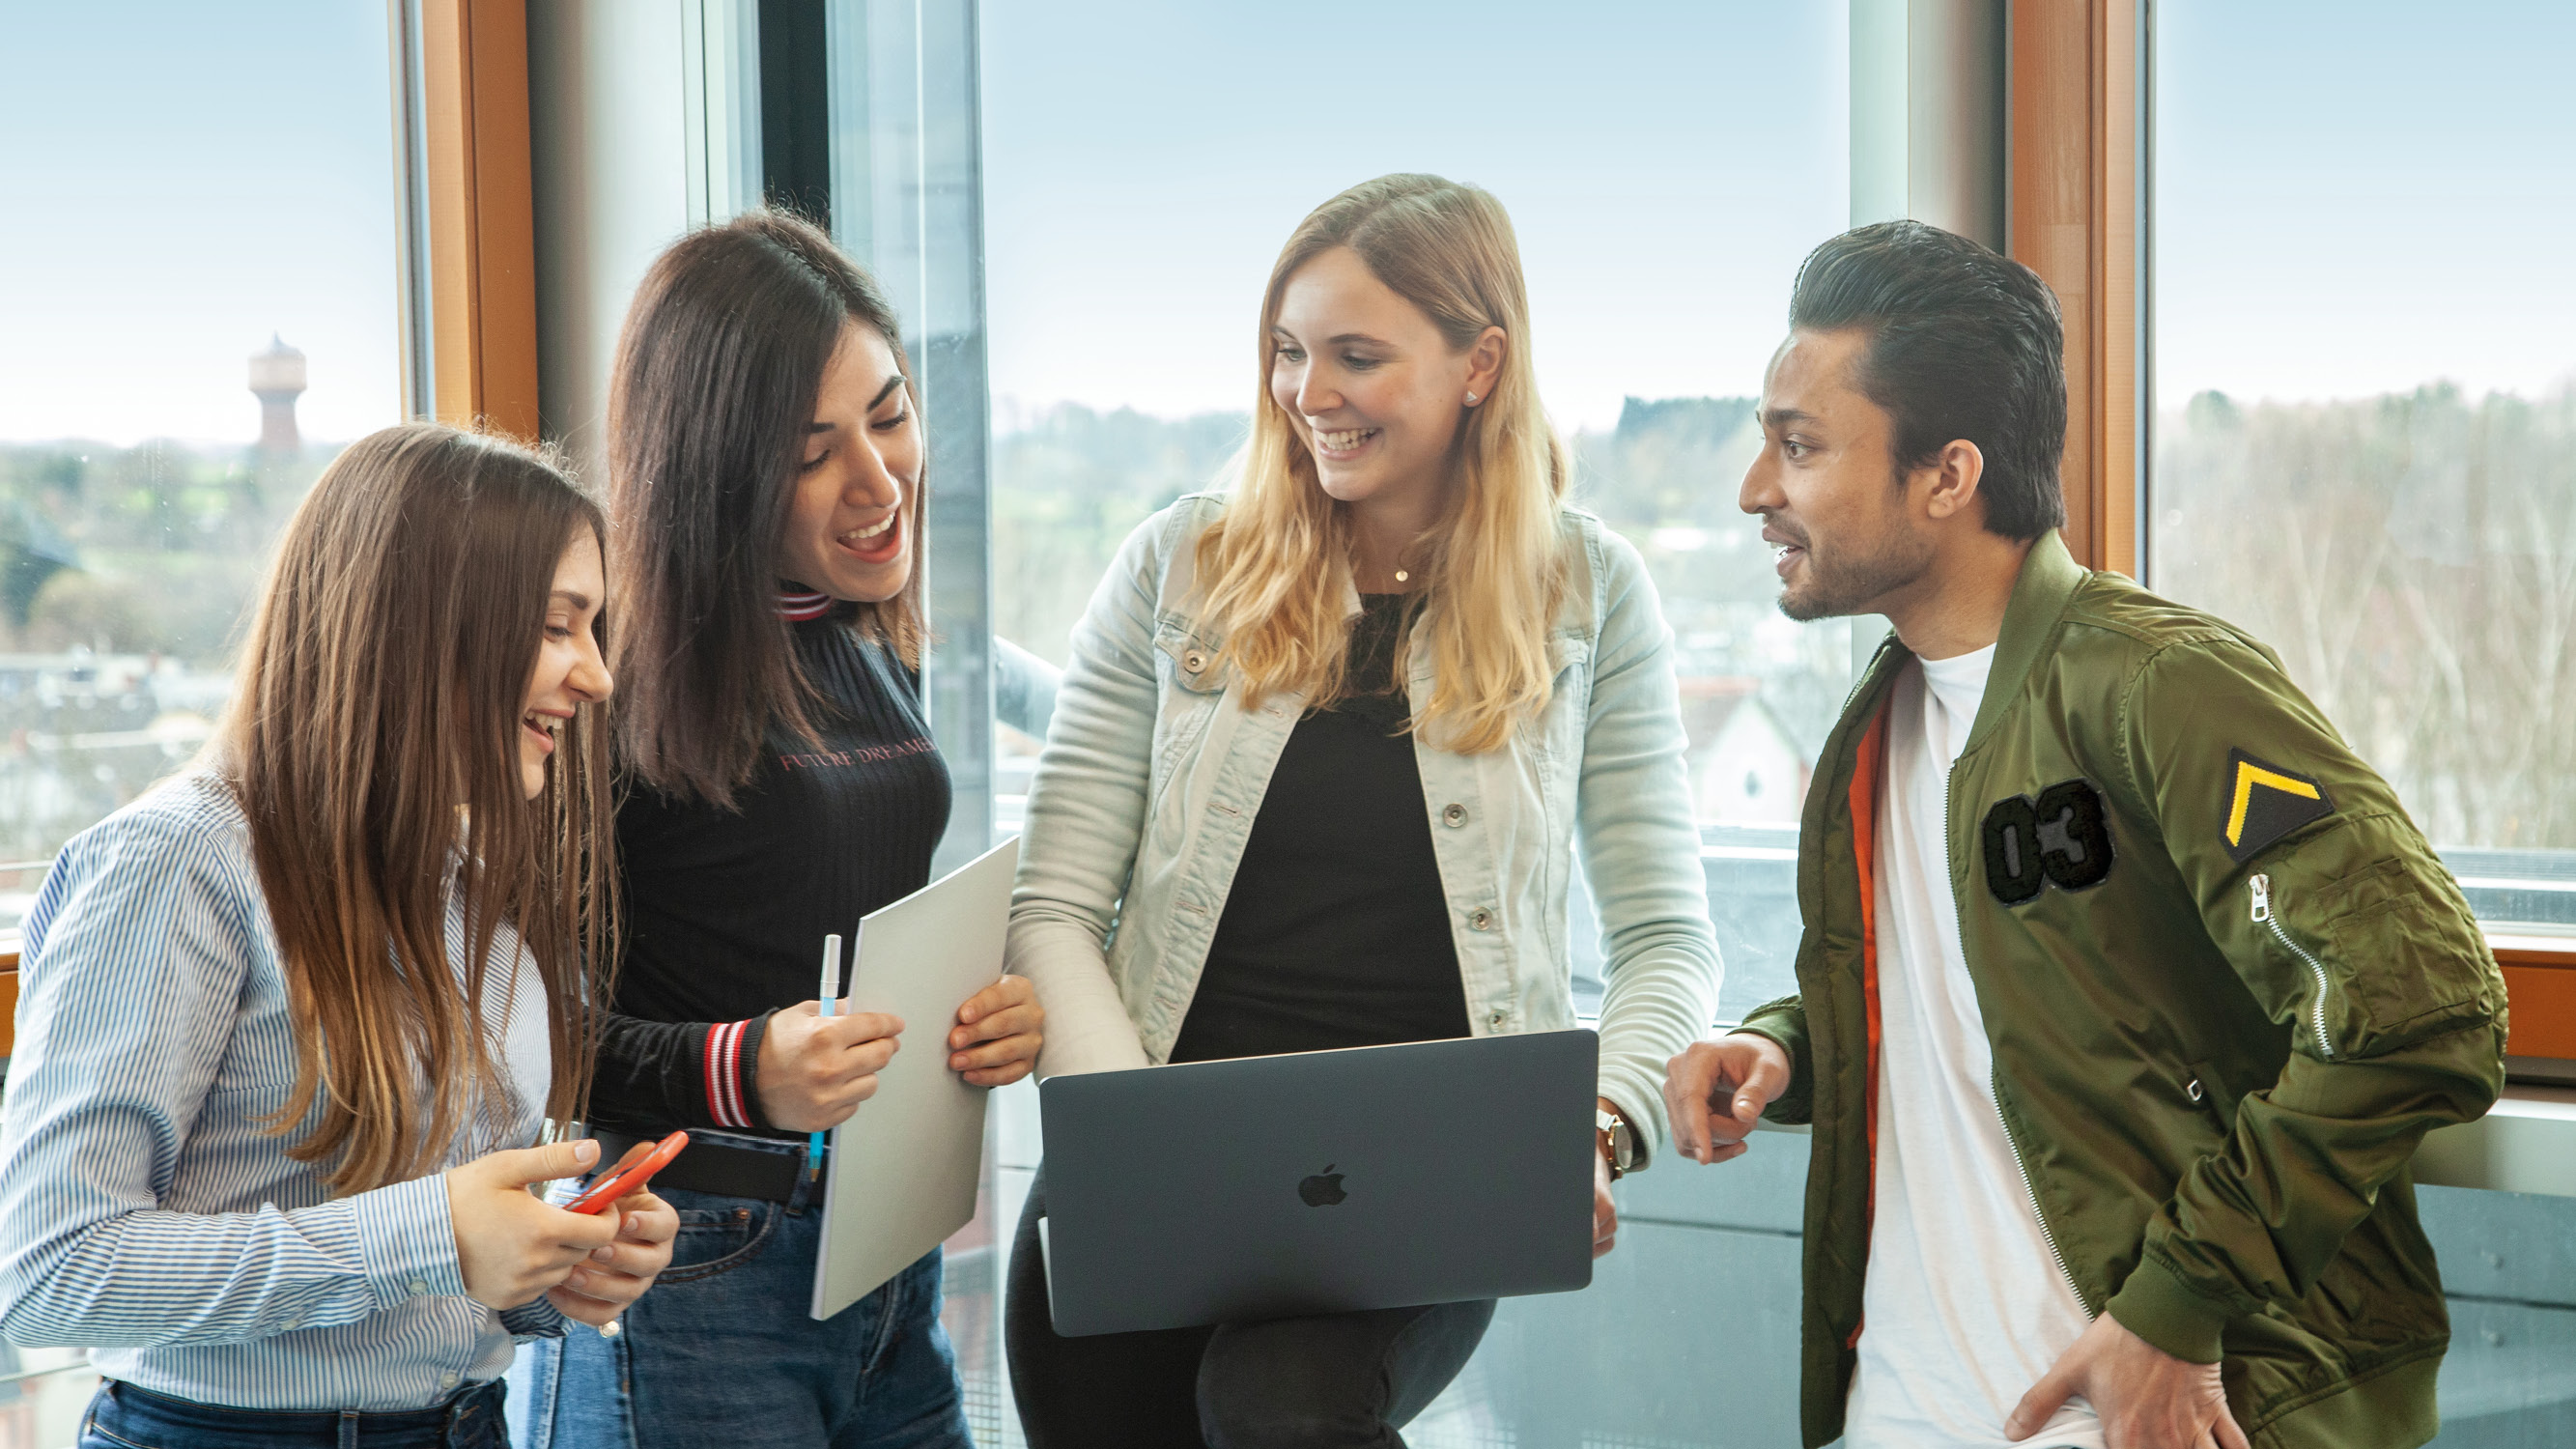
\includegraphics[width=\textwidth]{figures/thankyou.jpg}
			\captionof{figure}{Das Bild der Danke-Seite}
			\label{fig:thankyou}
		\end{column}
	\end{columns}
\end{frame}


% Folie – Grundlagen: Typische Schwachstellen (OWASP Top 10)
\begin{frame}{Grundlagen – Typische Schwachstellen (OWASP Top 10)}
	\begin{itemize}
		\item \textbf{A01 – Broken Access Control}  
		\begin{itemize}
			\item Fehlende oder fehlerhafte Zugriffsbeschränkungen
			\item z. B. Manipulation von JWT, IDOR
		\end{itemize}
		
		\item \textbf{A02 – Cryptographic Failures}  
		\begin{itemize}
			\item Unsichere oder falsch eingesetzte Verschlüsselung
			\item z. B. schwache Hashes, Klartextübertragung
		\end{itemize}
		
		\item \textbf{A03 – Injection}  
		\begin{itemize}
			\item Unsichere Eingabevalidierung $\rightarrow$ Angriffe möglich
			\item z. B. SQL Injection, Cross-Site Scripting (XSS)
		\end{itemize}
	\end{itemize}
\end{frame}


% Folie – Grundlagen: Privilege Escalation
\begin{frame}{Grundlagen – Privilege Escalation}
	\begin{itemize}
		\item \textbf{Ziel:} unberechtigter Zugriff auf höhere Rechte (Admin/Root)
		\item Häufig in Post-Exploitation-Phase
		\item \textbf{Typische Techniken (nach MITRE ATT\&CK):}
		\begin{itemize}
			\item Exploitation von Systemschwachstellen (T1068)
			\item Missbrauch von Sudo/SetUID (T1548)
			\item Manipulation von Zugriffstokens (T1134)
			\item Nutzung gültiger, privilegierter Accounts (T1078)
		\end{itemize}
	\end{itemize}
\end{frame}



% Folie – Grundlagen: Künstliche Intelligenz & LLMs
\begin{frame}{Grundlagen – Künstliche Intelligenz \& LLMs}
	\begin{itemize}
		\item \textbf{KI:} Mustererkennung, Automatisierung, Entscheidungsunterstützung
		\item \textbf{Maschinelles Lernen (ML):}
		\begin{itemize}
			\item Überwachtes Lernen (z. B. Klassifikation)
			\item Unüberwachtes Lernen (z. B. Anomalieerkennung)
			\item Bestärkendes Lernen (adaptives Verhalten)
		\end{itemize}
		\item \textbf{Large Language Models (LLMs):}
		\begin{itemize}
			\item Zerlegen komplexer Aufgaben in Schritte
			\item Generieren von Exploit-Vorschlägen \& Payloads
			\item Automatisierte Dokumentation
		\end{itemize}
		\item \textbf{Schwächen:} Halluzinationen, begrenztes Kontextfenster, fehlende Security-Spezialisierung
	\end{itemize}
\end{frame}


% Folie – Methodik: Toolauswahl
\begin{frame}{Methodik – Toolauswahl}
	\begin{itemize}
		\item \textbf{RamiGPT}
		\begin{itemize}
			\item Speziell für Privilege Escalation (Linux/Windows)
			\item Kombination von KI-Logik \& Tools wie LinPEAS, BeRoot
		\end{itemize}
		
		\item \textbf{PentestGPT (CLI)}
		\begin{itemize}
			\item Open-Source, textbasiert, strukturierte Workflows
			\item Unterstützt systematische Web-Pentest-Phasen
		\end{itemize}
		
		\item \textbf{PentestGPT (Web)}
		\begin{itemize}
			\item Kommerziell, dialogorientiert, direkte Nutzung im Browser
			\item Eignet sich für schnelle Ad-hoc-Analysen
		\end{itemize}
	\end{itemize}
\end{frame}


% Folie 9 – Testumgebungen
\begin{frame}{Testumgebungen}
	\begin{itemize}
		\item 3 VMs (Kali, Parrot, Ubuntu)
		\item OWASP Juice Shop (Web-Testumgebung)
		\item Isoliert \& reproduzierbar
	\end{itemize}
\end{frame}

% Folie 10 – Bewertungsmatrix
\begin{frame}{Bewertungsmatrix}
	\begin{itemize}
		\item 6 Kriterien:
		\begin{itemize}
			\item Schwachstellenabdeckung
			\item Exploit-Vorschläge
			\item Automatisierungsgrad
			\item Kontextverständnis
			\item Reporting
			\item Kosten-Nutzen
		\end{itemize}
	\end{itemize}
\end{frame}

% Folie – RamiGPT: Szenario
\begin{frame}{RamiGPT – Szenario}
	\begin{itemize}
		\item \textbf{Ziel:} Privilege Escalation unter Linux (Root-Rechte erlangen)
		\item \textbf{Setup:} Ubuntu-VM mit absichtlich fehlerhafter SetUID-Konfiguration (\enquote{rootbash})
		\item \textbf{Testmodus:}
		\begin{itemize}
			\item Full-AI (komplett automatisch)
			\item Halb-automatisch (mit manueller Unterstützung)
		\end{itemize}
	\end{itemize}
\end{frame}

% Folie – RamiGPT: Ergebnisse
\begin{frame}{RamiGPT – Ergebnisse}
	\begin{itemize}
		\item \textbf{Full-AI-Modus:}
		\begin{itemize}
			\item scheiterte an sudo-Passwortabfrage
			\item erkannte \enquote{rootbash} nicht eigenständig
		\end{itemize}
		
		\item \textbf{Halb-automatischer Modus:}
		\begin{itemize}
			\item mit manuellen Eingaben erfolgreich
			\item Privilege Escalation durch rootbash möglich
		\end{itemize}
		
		\item \textbf{Fazit:}  
		Nur mit Benutzerhilfe nutzbar, geringe Automatisierung
	\end{itemize}
\end{frame}


% Folie – PentestGPT (CLI): Szenarien
\begin{frame}{PentestGPT (CLI) – Szenarien}
	\begin{itemize}
		\item \textbf{Zielsystem:} OWASP Juice Shop (verwundbare Web-App)
		
		\item \textbf{Testschwerpunkte (OWASP Top 10):}
		\begin{itemize}
			\item Broken Access Control → JWT-Manipulation, IDOR
			\item Cryptographic Failures → unsichere Hashes, \enquote{Weird Crypto}-Challenge
			\item Injection → SQLi, DOM-basiertes XSS
		\end{itemize}
		
		\item \textbf{Interaktion:}
		\begin{itemize}
			\item Strukturierte Workflows über CLI-Befehle (\texttt{next}, \texttt{more}, \texttt{discuss})
			\item GPT-gestützte Vorschläge, manuelle Ausführung durch Nutzer
		\end{itemize}
	\end{itemize}
\end{frame}


% Folie – PentestGPT (CLI): Ergebnisse
\begin{frame}{PentestGPT (CLI) – Ergebnisse}
	\begin{itemize}
		\item \textbf{Stärken:}
		\begin{itemize}
			\item Liefern valider Payloads (z. B. \texttt{' OR '1'='1} $\rightarrow$ Login-Bypass, Admin-Zugriff)
			\item Systematische Struktur → didaktisch wertvoll (Ausbildung, Training)
			\item Gute Unterstützung bei IDOR \& XSS durch Payload-Beispiele
		\end{itemize}
		
		\item \textbf{Schwächen:}
		\begin{itemize}
			\item Keine echte Automatisierung $\rightarrow$  alles manuell auszuführen
			\item Teilweise generische Antworten, Detailtiefe nur mit Nachfragen
			\item Kein Reporting-Export, nur Logfiles
		\end{itemize}
		
		\item \textbf{Fazit:}  
		Hilfreiches Assistenztool, besonders für strukturierte Tests und Ausbildung
	\end{itemize}
\end{frame}













% Folie – PentestGPT (Web): Szenarien
\begin{frame}{PentestGPT (Web) – Szenarien}
	\begin{itemize}
		\item \textbf{Zielsystem:} OWASP Juice Shop (wie CLI-Version)
		
		\item \textbf{Testschwerpunkte:}
		\begin{itemize}
			\item Broken Access Control (z. B. JWT-Manipulation, IDOR)
			\item Cryptographic Failures (\enquote{Weird Crypto})
			\item Injection (SQLi, XSS)
		\end{itemize}
		
		\item \textbf{Interaktion:}
		\begin{itemize}
			\item Dialogorientiert, ähnlich wie ChatGPT
			\item Prompts in natürlicher Sprache (DE \& EN)
			\item Schnelle Ad-hoc-Analysen im Browser
		\end{itemize}
	\end{itemize}

\end{frame}

% Folie – PentestGPT (Web): Ergebnisse
\begin{frame}{PentestGPT (Web) – Ergebnisse}
	\begin{itemize}
		\item \textbf{Stärken:}
		\begin{itemize}
			\item Schnelle \& präzise Antworten $\rightarrow$ sofort Exploit-Beispiele
			\item Einfache Bedienung, keine Installation notwendig
			\item Kontextsensitiv (Deutsch/Englisch kein Unterschied)
		\end{itemize}
		
		\item \textbf{Schwächen:}
		\begin{itemize}
			\item Keine Automatisierung $\rightarrow$ alles manuell auszuführen
			\item Kein Reporting-Export, Ergebnisse nur im Chat
			\item Volle Funktionen nur in kostenpflichtiger Version
		\end{itemize}
		
		\item \textbf{Fazit:}  
		Praktisch für schnelle Analysen \& Proof-of-Concepts, weniger für strukturierte Tests
	\end{itemize}
\end{frame}

% Folie – Vergleich der Tools
\begin{frame}{Vergleich der Tools}
	\begin{itemize}
		\item \textbf{Bewertungskriterien:}  
		Schwachstellenabdeckung, Exploit-Vorschläge, Automatisierung, Kontextverständnis, Reporting, Kosten-Nutzen
		
		\item \textbf{Gesamtpunkte (max. 12):}
		\begin{itemize}
			\item RamiGPT: 5/12
			\item PentestGPT (CLI): 8/12
			\item PentestGPT (Web): 7/12
		\end{itemize}
		
		\item \textbf{Stärken \& Schwächen:}
		\begin{itemize}
			\item RamiGPT: interessant für Privilege Escalation, aber unreif, wenig Automatisierung
			\item CLI: methodisch klar, gute Payloads, aber langsamer \& manuell
			\item Web: schnell \& flexibel, aber limitiert ohne Automatisierung/Reporting
		\end{itemize}
	\end{itemize}
\end{frame}

% Folie – Stärken & Schwächen der KI-Tools
\begin{frame}{Stärken \& Schwächen der KI-Tools}
	\begin{columns}[T,onlytextwidth]
		% Linke Spalte: Stärken
		\begin{column}{0.48\textwidth}
			\textbf{Stärken}
			\begin{itemize}
				\item Unterstützung bei Routineaufgaben (z. B. Payload-Generierung)
				\item Nützliche Exploit-Vorschläge und Erklärungen
				\item Methodische Unterstützung (CLI) bzw. schnelle Ad-hoc-Analysen (Web)
				\item Niedrige Einstiegshürden für Einsteiger \& Ausbildung
			\end{itemize}
		\end{column}
		
		% Rechte Spalte: Schwächen
		\begin{column}{0.48\textwidth}
			\textbf{Schwächen}
			\begin{itemize}
				\item Geringe Automatisierung $\rightarrow$  keine End-to-End-Pentests
				\item Schwaches Kontextverständnis (z. B. RamiGPT bei Passwortabfragen)
				\item Ergebnisse oft nicht reproduzierbar
				\item Fehlende Reporting-/Exportfunktionen
			\end{itemize}
		\end{column}
	\end{columns}
\end{frame}

% Folie – Fazit
\begin{frame}{Fazit}
	\begin{itemize}
		\item \textbf{KI = Unterstützung, kein Ersatz}  
		→ menschliche Expertise bleibt unverzichtbar
		
		\item \textbf{Nutzen:}
		\begin{itemize}
			\item Effizienzsteigerung bei Routineaufgaben
			\item Hilfreich für Ausbildung \& strukturierte Analysen
			\item Schnelle Proof-of-Concepts möglich
		\end{itemize}
		
		\item \textbf{Grenzen:}
		\begin{itemize}
			\item Keine vollständige Automatisierung
			\item Ergebnisse nicht immer reproduzierbar
			\item Eingeschränktes Kontextverständnis
		\end{itemize}
	\end{itemize}
\end{frame}


% Folie – Ausblick
\begin{frame}{Ausblick}
	\begin{itemize}
		\item \textbf{Integration in DevSecOps}  
		→ KI-gestützte Tools als Teil kontinuierlicher Sicherheitsprozesse
		
		\item \textbf{Technische Weiterentwicklung}  
		→ Größere Kontextfenster \& verbesserte Modelle  
		→ Retrieval-Augmented Generation (RAG) für aktuelles Wissen
		
		\item \textbf{Anwendung in der Ausbildung}  
		→ KI als interaktiver Trainingspartner  
		→ Unterstützung beim Erlernen von Angriffstechniken \& Abwehrmaßnahmen
		
		\item \textbf{Langfristige Perspektive}  
		→ KI erweitert klassische Pentests  
		→ Richtung: skalierbare \& adaptive Sicherheitsprüfungen
	\end{itemize}
\end{frame}


















%
%%%%%%%%%%%%%%%%%%%%%%%%%%%%%%%%%%%%%%%%%%%%%%%%%%%%%%%%%%%%
%	\section{Grundlegende Verwendung}
%
%	\begin{frame}[fragile]{Allgemeines zur Verwendung}{Minimalbeispiel}
%		Der folgende Ausschnitt erzeugt Ihnen eine neue, leere Präsentation im Stil der Hochschule (ohne spezifische Fakultät) mit den Standardoptionen:
%
%		\scriptsize
%		\begin{verbatim}
%		\documentclass[aspectratio=169,onlytextwidth,t]{beamer}
%		\usetheme{hsmw}
%
%		\title[Kurztitel für Fußzeile]{Titel der Präsentation für Titelseite}
%		\subtitle{Untertitel für Titelseite}
%		\author{Name Vortragende(r)}
%		\date{Datum der Präsentation}
%
%		\begin{document}
%			\begin{frame}{Erste Folie}
%				Inhalt
%			\end{frame}	
%		\end{document}
%		\end{verbatim}
%	\end{frame}
%
%	\begin{frame}[fragile]{Mögliche Optionen (1/3)}{Grundlegende Stilelemente beeinflussen}
%		Sie können grundlegende Stilelemente über die Angabe von Optionen beim Laden des \textit{Beamer-Themes} (\texttt{\textbackslash{}usetheme[\textcolor{hsmw}{optionen}]\{hsmw\}}) beeinflussen:
%		\begin{itemize}
%			\item Allgemeine Anpassungen (Farben und Texte):
%			\begin{itemize}
%				\item Farbschema:
%				\begin{itemize}
%					\item Standardeinstellung Hochschul-Blau: \textcolor{hsmw}{hs}, \textcolor{hsmw}{inst} oder \textit{<leer>}
%					\item Fakultäts-Farben: \textcolor{hsmw}{inw}, \textcolor{hsmw}{cb}, \textcolor{hsmw}{me}, \textcolor{hsmw}{sw}, \textcolor{hsmw}{wi}
%					\item Alternative Schreibweise: \textcolor{hsmw}{faculty=inw}, \textcolor{hsmw}{faculty=cb}, \dots
%				\end{itemize}
%
%				\item Sprache (Ändert einige Bezeichner, z.\,B. Fakultätsnamen, Datumsformat, \dots): 
%				\begin{itemize}
%					\item Standardeinstellung Deutsch: \textcolor{hsmw}{language=ngerman} oder \textit{<leer>}
%					\item Englisch: \textcolor{hsmw}{language=english}
%					\item Andere Sprachen sind möglich, aber noch nicht implementiert (bei Interesse melden!)
%				\end{itemize}
%			\end{itemize}
%
%			\item Individuelle Anpassungen an den eigenen Geschmack:
%			\begin{itemize}
%				\item \textcolor{hsmw}{toc} fügt ein Inhaltsverzeichnis nach der Titelseite ein
%				\item \textcolor{hsmw}{sectionslide} fügt eine zusätzliche Seite für jede \verb!\section! ein
%			\end{itemize}
%		\end{itemize}
%	\end{frame}
%
%	\begin{frame}[fragile]{Mögliche Optionen (2/3)}{Grundlegende Stilelemente beeinflussen}
%		\begin{itemize}
%			\item[] \textcolor{hsmwLightGray}{Individuelle Anpassungen an den eigenen Geschmack (Fortsetzung):}
%			\begin{itemize}
%				\item \textcolor{hsmw}{subsectionslide} fügt eine zusätzliche Seite für jede \verb!\subsection! ein.\newline
%					(kombinierbar mit \textcolor{hsmw}{sectionslide})
%				\item \textcolor{hsmw}{smallpagenumber} reduziert die Größe der Foliennummer
%				\item \textcolor{hsmw}{nototalpages} verbirgt die Gesamtzahl der Folien neben der Foliennummer
%				\item \textcolor{hsmw}{nofacultyicon} verbirgt das Fakultäts-Icon auf der Titelseite
%				\item \textcolor{hsmw}{colormath} hebt mathematische Formeln farbig ab
%				\begin{itemize}
%					\item Keine Hervorhebung: \textcolor{hsmw}{colormath=off} oder \textit{<leer>}
%					\item Formeln sind hervorgehoben, aber Text in Formeln mittels \verb!\text{...}! wird wie normaler Text dargestellt: \textcolor{hsmw}{colormath=nottext} oder \textcolor{hsmw}{colormath}
%					z.\,B.
%					\[\sum^n_{k=0} k = \frac{n(n+1)}2 \qquad \text{ für }  n \in\mathbb N\]
%					\item Vollständige Hervorhebung: \textcolor{hsmw}{colormath=full}
%				\end{itemize}
%			\end{itemize}
%		\end{itemize}
%	\end{frame}
%	
%	\begin{frame}[fragile]{Mögliche Optionen (3/3)}{Grundlegende Stilelemente beeinflussen}
%		\begin{itemize}
%			\item[] \textcolor{hsmwLightGray}{Individuelle Anpassungen an den eigenen Geschmack (Fortsetzung):}
%			\begin{itemize}
%				\item \textcolor{hsmw}{printhandout} setzt zwei Folien pro A4-Seite (Klassenoption \textit{handout} notwendig)
%				\item \textcolor{hsmw}{noframesubtitle} deaktiviert alle Untertitel der Folien (vergrößert Textbereich)
%			\end{itemize}
%			\item Zusätzliche Optionen (nicht ganz konform mit dem Corporate Design):
%			\begin{itemize}
%				\item \textcolor{hsmw}{titlepagedate} zeigt das Datum auf der Titelseite
%				\item \textcolor{hsmw}{fancystyle} aktiviert einige Farbanpassungen
%				\item \textcolor{hsmw}{progressbar} zeigt einen Fortschrittsbalken am unteren Rand der Folien
%			\end{itemize}
%		\end{itemize}
%
%		\vspace*{\baselineskip}
%		\textbf{Beispiele:}
%		\begin{itemize}
%			\item \verb!\usetheme[toc, sectionslide, nofacultyicon]{hsmw}!
%			\item \verb!\usetheme[cb, colormath, progressbar]{hsmw}!
%			\item \verb!\usetheme[faculty=wi, colormath]{hsmw}!
%		\end{itemize}
%	\end{frame}
%
%
%	
%	\begin{frame}[fragile]{Erweitertes Beispiel (Stil: Fakultät CB)}{Mit ein paar zusätzlichen Optionen und Befehlen}
%		\scriptsize
%		\begin{verbatim}
%			\documentclass[aspectratio=169,onlytextwidth,t]{beamer}
%			\usetheme[cb, colormath]{hsmw}
%			
%			\title[Kurztitel für Fußzeile]{Titel der Präsentation für Titelseite}
%			\subtitle{Untertitel für Titelseite}
%			\author{Name Vortragende(r)}
%			\email{E-Mail}
%			\titlegraphic{figures/thankyou.jpg}
%
%			\begin{document}
%				\begin{frame}{Erste Folie}{Mit Untertitel}
%					Inhalt
%				\end{frame}	
%
%				\appendix
%				\makethankyou
%			\end{document}
%		\end{verbatim}
%	\end{frame}
%
%	\begin{frame}{Anwendungshinweise}{Was es zu beachten gilt}
%		\begin{itemize}
%			\item Für die Verwendung in lokalen TeX-Distributionen oder auch Overleaf geeignet
%
%			\item Verzeichnisstruktur für das Auffinden der Dateien notwendig
%			\begin{itemize}
%				\item Funktionen und Aufbau auf mehrere Quelldateien verteilt
%				\begin{itemize}
%					\item beamerthemehsmw.sty: Optionen, Pakete und Macros (lädt die restlichen Dateien)
%					\item beamerouterthemehsmw.sty: Allgemeine Layout-Einstellungen (Folientitel, Fußzeilen, ...)
%					\item beamerinnerthemehsmw.sty: Inhaltsbezogene Layout-Einstellungen (Titelseite, Aufzählungen, ...)
%					\item beamerfontthemehsmw.sty: Die verwendeten Schriftstile und -größen
%					\item beamercolorthemehsmw*.sty: Das spezifische Farbschema für die einzelnen Elemente (inkl. Fakultätsfarben)
%				\end{itemize}
%
%				\item Unterverzeichnis für zusätzliches Bildmaterial: ./figures/*
%			\end{itemize}
%		\end{itemize}
%	\end{frame}
%
%	\begin{frame}{Besonderheiten}{Eventuelle Probleme, die gar keine sind}
%		\begin{itemize}
%			\item Bei überlangen (Unter-)Titeln auf der Titelseite und auf den Folien wird bei Bedarf die Schriftgröße heruntergesetzt
%			\item Sie erhalten dafür eine Paket-Warnung in der Logdatei, die Sie darauf hinweist:
%			\newline
%			\resizebox{\linewidth}{!}{\enquote{Package beamerinnerthemehsmw Warning: Font of text '\textit{<text>}' is scaled down by a factor of \textit{<factor>}}}
%			\item Sie können diese Texte ggf. anpassen, damit sie nicht skaliert werden müssen
%			\item Sie können den Warnhinweis allerdings auch einfach ignorieren
%		\end{itemize}
%	\end{frame}
%
%	\section{Inhalte gestalten}
%
%	\begin{frame}{Eine normale Folie mit Fließtext}{... und einem Untertitel}
%		\blindmathtrue
%		\blindtext
%	\end{frame}
%
%	\begin{frame}[c]{Eine normale Folie vertikal zentriert}{Unter Verwendung der Folien-Option: \texttt{\textbackslash{}begin\{frame\}[c] ... \textbackslash{}end\{frame\}}}
%		\blindmathtrue
%		\blindtext
%	\end{frame}
%
%	\begin{frame}[b]{Eine normale Folie unten ausgerichtet}{Unter Verwendung der Folien-Option: \texttt{\textbackslash{}begin\{frame\}[b] ... \textbackslash{}end\{frame\}}}
%		\blindmathtrue
%		\blindtext
%	\end{frame}
%	
%	\begin{frame}{Eine Folie mit zwei Spalten}{Einfache Mathematik: Mehr Spalten = mehr Platz}
%		\begin{columns}
%			\begin{column}[T]{.5\textwidth}
%				\blindlistlist[3]{itemize}[3]
%			\end{column}
%			\begin{column}[T]{.5\textwidth}
%				\blindlistlist[2]{itemize}[4]
%			\end{column}
%		\end{columns}
%	\end{frame}
%
%	\begin{frame}{Eine Folie mit zwei Spalten}{Auch passend für Abbildungen}
%		\begin{columns}
%			\begin{column}[T]{.5\textwidth}
%				\blindlistlist[3]{itemize}[3]
%			\end{column}
%			\begin{column}[T]{.5\textwidth}
%				\centering
%				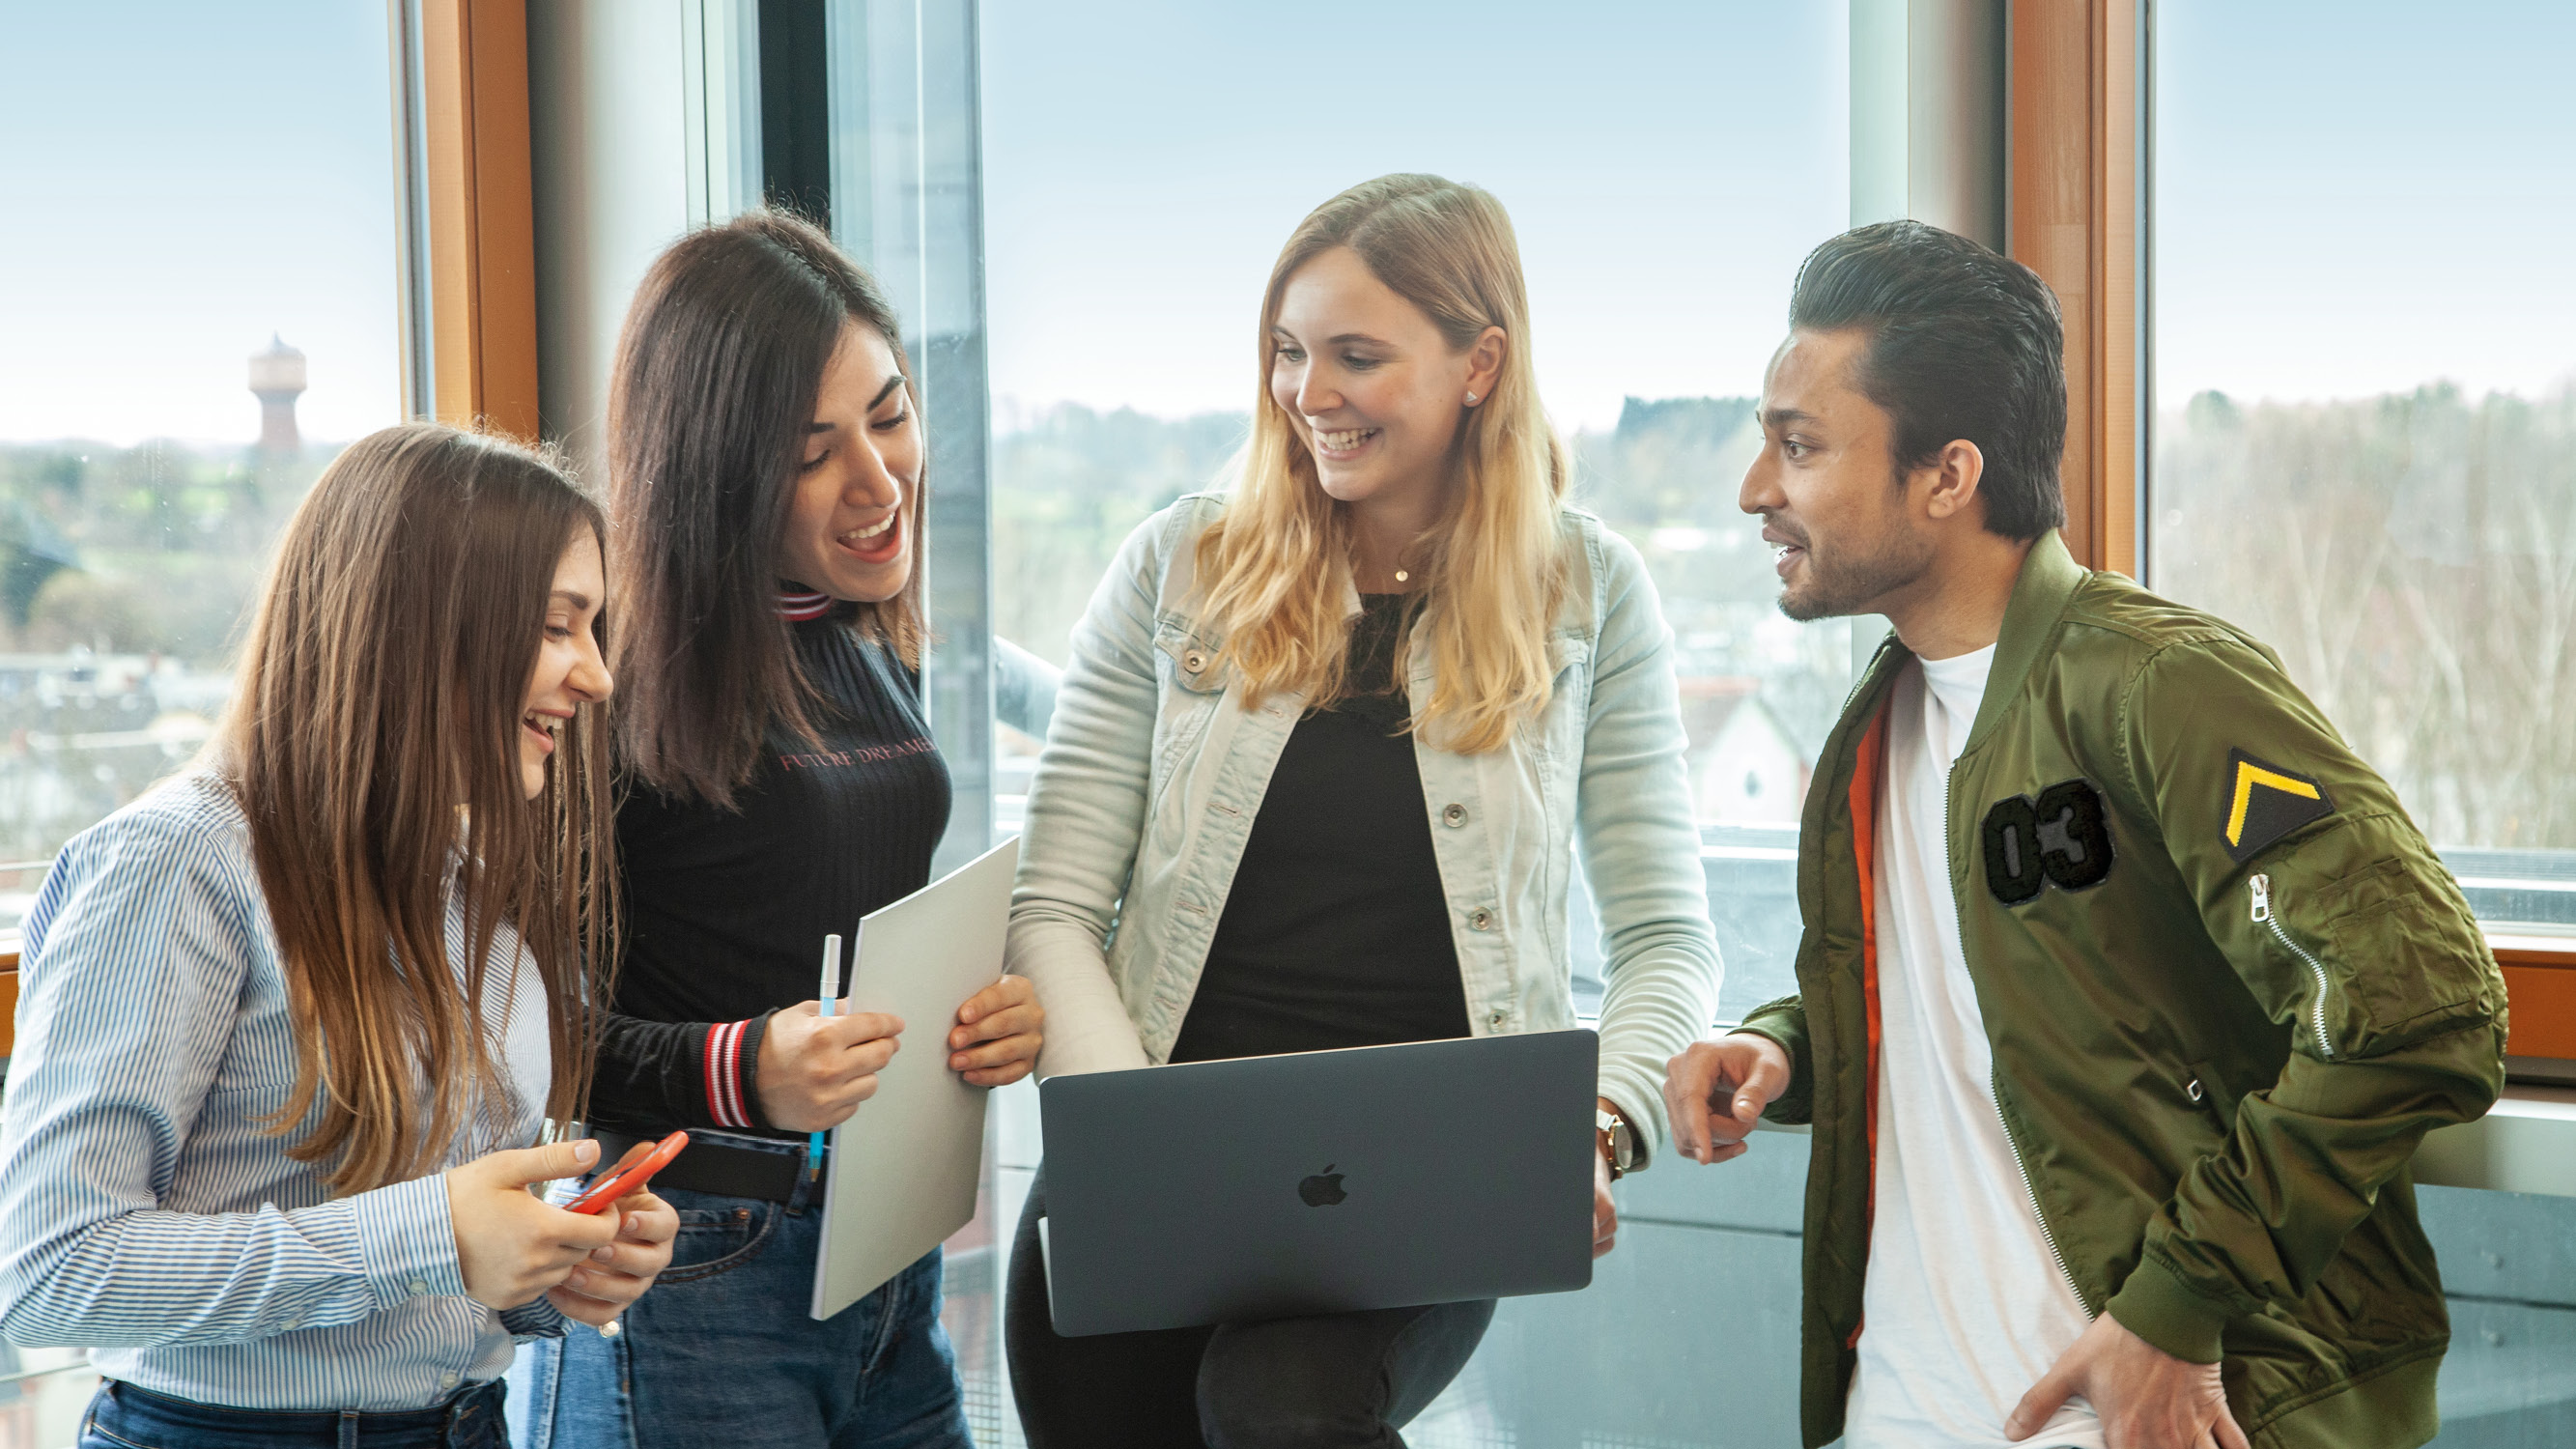
\includegraphics[width=\textwidth]{figures/thankyou.jpg}
%				\captionof{figure}{Das Bild der Danke-Seite}
%				\label{fig:thankyouq}
%			\end{column}
%		\end{columns}
%	\end{frame}
%
%	\begin{frame}[fragile]{Inhalte absolut positionieren}
%		\begin{itemize}
%			\item Der Koordinatenursprung für ist die obere linke Ecke
%			\item Koordinatensystem in Zentimetern, an Seitenverhältnis 16:9 ausgerichtet
%			\begin{itemize}
%				\item $ 0 \le x \le 16 $
%				\item $ 0 \le y \le 9 $
%			\end{itemize}
%
%			\item Verwendung von \verb!begin{textblock}{breite}(x-pos, y-pos)!...
%		\end{itemize}
%
%		\begin{textblock}{5}(10, 4.5)
%			\scriptsize
%			\begin{verbatim}
%				\begin{textblock}{5}(10, 4.5)
%					Inhalt
%				\end{textblock}
%			\end{verbatim}
%		\end{textblock}
%
%		\begin{textblock}{15}(0.5, 6)
%			\hrule
%			\scriptsize
%			\begin{verbatim}
%				\begin{textblock}{15}(0.5, 6)
%					\hrule
%				\end{textblock}
%			\end{verbatim}
%		\end{textblock}
%	\end{frame}
%
%	\begin{frame} 
%		\frametitle{Mehrere Folien mittels \textit{Overlays}} 
%		\begin{theorem}
%			Es gibt keine \enquote{größte} Primzahl.
%		\end{theorem} 
%		\begin{enumerate} 
%			\item<1-| alert@1> Angenommen $p$ wäre die größte Primzahl.
%			\item<2-> Sei $q$ das Produkt der ersten $p$ Zahlen. 
%			\item<3-> Dann ist $q+1$ durch keine davon teilbar.
%			\item<4-> Aber $q + 1$ ist größer als $1$ und daher durch eine Primzahl teilbar, die nicht in den ersten $p$ Zahlen liegt.
%		\end{enumerate}
%
%		\uncover<3->{\scriptsize Hinweis: Mathe ist super kompliziert!}
%
%		\vfill
%		\only<2,4>{\centering\textbf{Achtung}: Besonders wichtiger Schritt!}
%		\vfill
%	\end{frame}
%
%	\section{Benutzerdefinierte Anpassungen}
%
%	\newcommand{\rgb}[1]{\textcolor{hsmw80}{#1}}
%	\newcommand{\cmd}[1]{\rgb{\textbackslash{}#1}}
%	\newcommand{\textto}{\hspace*{0.2ex}\tikz[baseline=-.33em] \draw[-latex] (0,0) to ++(2ex, 0);\hspace*{0.2ex}}
%	\begin{frame}{Zusätzliche, beeinflussbare Macros}{... und deren Abhängigkeiten (zur Feinabstimmung der eigenen Präsentation)}
%		\begin{itemize}
%			\item Option \rgb{hs}, \rgb{cb}, ... oder \rgb{faculty=cb, me, ...} (Farbschema)
%			\begin{itemize}
%				\item \cmd{insertfacultyicon} (Titelseite)
%				\item \cmd{insertfacultyname} (Option \rgb{language}) \textto{} \cmd{institute\{\cmd{insertfacultyname}\}}
%			\end{itemize}
%			\item \cmd{insertthankyoutitle}, \cmd{insertthankyoutext}, \cmd{insertthankyousidebartext}
%			\begin{itemize}
%				\item \cmd{email} \textto{} \cmd{insertemail}
%				\item \cmd{phone} \textto{} \cmd{insertmobilephone}, \cmd{inserttelephone}
%				\item \cmd{office} \textto{} \cmd{insertoffice}
%				\item \cmd{courseofstudies} \textto{} \cmd{insertcourseofstudies}
%				\item \cmd{additional} \textto{} \cmd{insertadditionalsidebar}, \cmd{insertadditional}
%			\end{itemize}
%			\item \cmd{setcurrentspeaker}, \cmd{resetcurrentspeaker} (\cmd{insertshortauthor})
%			\begin{itemize}
%				\item Stern-Version (\cmd{setcurrentspeaker*}) setzt zusätzlich Label (Option \rgb{language})
%				\item \cmd{currentspeaker} (\cmd{currentspeakerlabel}) \textto{} \cmd{insertcurrentspeaker}
%			\end{itemize}
%		\end{itemize}
%	\end{frame}
%
%	\section{FAQ}
%
%	\begin{frame}[c]{FAQ: Häufig gestellte Fragen}{Hier ist noch Platz für Anwendungsfälle oder Antworten auf häufig gestellte Fragen}
%		Es sind alle zum Testen und zur Übermittlung von konstruktivem Feedback eingeladen!
%		\\[\baselineskip]
%		Bei Ideen, Wünschen, Anregungen, Fragen und auch Problemen:
%		\begin{itemize}
%			\item Offizielle LaTeX-GitLab-Gruppe der Hochschule Mittweida:
%			\newline
%			\href{https://git.hs-mittweida.de/hsmw-latex}{git.hs-mittweida.de/hsmw-latex}
%
%			\item Kontaktieren Sie mich gern per E-Mail \href{mailto:schildba@hs-mittweida.de?subject=[LaTeX] Beamer-Vorlage}{schildba@hs-mittweida.de}
%
%			\item Nutzen Sie einen der anderen verfügbaren Kommunikationskanäle
%		\end{itemize}
%	\end{frame}
%
	\appendix
	\appendix
	\section*{Literatur}
	
	\begin{frame}[allowframebreaks]{Literatur}
		\begin{thebibliography}{9}
			\bibitem{bitkom2023}
			Bitkom (2023): \\
			Mangel an IT-Fachkräften droht sich zu verschärfen. \\
			\url{https://www.bitkom.org/Presse/Presseinformation/Mangel-an-IT-Fachkraeften-droht-sich-zu-verschaerfen}
		\end{thebibliography}
	\end{frame}
	
	\makethankyou
%	\makebibliography
%
%	\section{\appendixname}
%
%	\begin{frame}{Zusätzliche Folien}{Der Anhang zählt nicht mit zu den regulären Folien}
%		\blindtext
%	\end{frame}

\end{document}
